\section{Methodology}

\subsection{\textbf{Echo State Networks}}
An ``echo state network'' (also
called a ``liquid state machine'' \cite{lukosevicius_practical_2012}) is a type
of recurrent neural network that uses a single layer of many neurons called a
``reservoir.'' The reservoir has an adjacency matrix $\bm{A}$ that
\begin{enumerate}
	\item is sparsely populated
	\item is connected by uniformly random weights centered at zero
	\item has a large number of neurons
\end{enumerate}
A reservoir computer also satisfies the \textit{echo state property}
\cite{pathak_model-free_2018, lukosevicius_reservoir_2009}. This
property ensures that a system's state has a decaying influence on future states
(like an echo of sound or ripples on water). This property is satisfied in most
cases when the the absolute value of the greatest eigenvalue of
$\bm{A}$ (the spectral radius, $\rho$) \cite{lukosevicius_reservoir_2009} is,
\begin{align}
	\rho(\bm{A}) < 1.
\end{align}
However, the echo state property can still be satisfied for a spectral radius
greater than unity \cite{lukosevicius_practical_2012}.

\begin{figure}[H]
	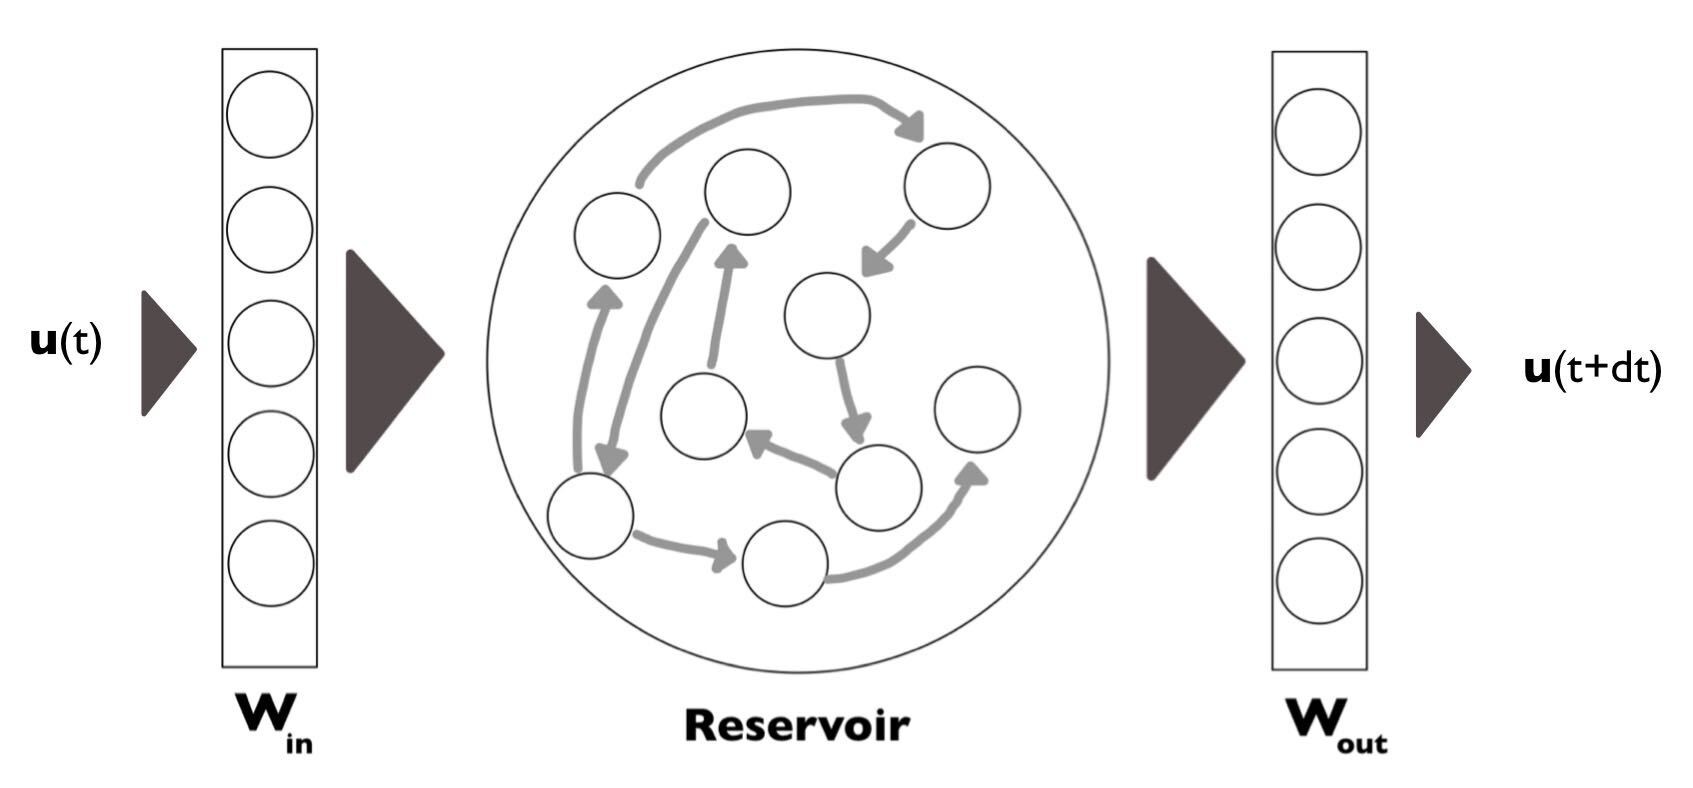
\includegraphics[width=\columnwidth]{reservoir_network.jpg}
	\caption{A basic reservoir computer or echo state network. The connections in
	the reservoir are given by $\bm{A}$}
	\label{fig:RCmodel}
\end{figure}

Figure \ref{fig:RCmodel} gives a visual representation of a basic
\acrshort{ESN}. An
input vector of length \textit{K} is mapped to the reservoir layer by an input
weight matrix $\bm{W_{in}}$. The state of the reservoir is mapped to an output
layer of length \textit{N} with an output weight matrix $\bm{W_{out}}$.
The output weight matrix is trained through
backpropagation using a loss function like cross entropy
\cite{pathak_model-free_2018, vlachas_backpropagation_2020}.

In this
work, the input vector is a function of time, $\bm{u}(t)$, and the output
vector is the next state of the system, $\bm{u}_p(t+\Delta t)$. Ideally, the
difference between the prediction, $\bm{u}_p$, and the actual, $\bm{u}_a$, is
minimized. \glspl{ESN} are capable of mapping an input vector of any size to
an output vector of any size. For example, $\bm{u}(t)$ could be the total
demand
at $t$ and $\bm{u}_p(t+\Delta t)$ could be the total demand at $t+\Delta t$. In
that scenario the reservoir is a one-to-one map. Alternatively, $\bm{u}(t)$
could be several data points, temperature, air pressure, irradiance, wind
speed, and total demand, at time $t$ and $\bm{u}_p(t+\Delta t)$ could be the
net demand at $t+\Delta t$. In this case the reservoir is a many-to-one map.
Determining the combination of input data that leads to the most accurate
predictions is a key area of research and an important part of this study
\cite{kobylinski_high-resolution_2020,bianchi_reservoir_2020}. For the results
shown below, $\bm{u}(t)$ is just the hourly demand.

\subsection{\textbf{Hyperparameter Search}}
Due to the architecture of \glspl{ESN}, the weights and connections
inside the reservoir do not need to be trained and, in our choice of
implementation, cannot be. This dramatically reduces the training time because
only the linear output layer needs to be trained. One drawback of this approach
is its sensitivity to hyperparameters, which must be carefully chosen before
running the network \cite{ pathak_model-free_2018,
lukosevicius_practical_2012, lukosevicius_reservoir_2009,gallicchio_deep_2019}.
Here, we perform grid searches
to establish which combination of hyperparameters minimizes the mean squared
error of the model,
\begin{align}
	MSE &= \frac{1}{N}\sum_i^N (\hat{y} - y_i)^2\\
	\intertext{where}
	\hat{y} &= \mbox{the average value of the ouput.}\nonumber
\end{align}

\subsection{\textbf{Constructing the \gls{ESN}}}

We constructed the \gls{ESN} in our initial demonstration with the open source
Python package \texttt{pyESN} \cite{korndorfer_pyesn_2015}. The code
is freely available on GitHub. Two models were trained with
historical demand data from \gls{uiuc} in 2017.  Each model had a
reservoir of 500 neurons. One was trained on 1000 hours of
data and predicted the following 100 hours of demand in two hour
increments. The other was trained on 3500 hours of data and, once again,
predicted the following 100 hours.

A grid search informed our choice of hyperparameters for these models, shown in
Figure \ref{fig:gridsearch}. This search determined the optimal combination of
spectral radius ($\rho$) and noise injection (for regularization of reservoir
neurons), shown in Figure \ref{fig:gridsearch}, following the recommendations
from \cite{lukosevicius_practical_2012}. Figure
\ref{fig:gridsearch} shows that there may be multiple combinations of
hyperparameters that give a low mean squared error. The hyperparameters that
will be used in future work reflect a global minimum in the parameter space
where $\rho = 1.3$ and \texttt{noise} $= 0.01$. 

\begin{figure}[h]
  \centering
  \includegraphics[width=0.8\columnwidth]{noise_spectral_radius.png}
  \caption{A grid search over a range of spectral radii and noise levels. The
  optimal set minimizes the mean squared error.}
  \label{fig:gridsearch}
\end{figure}
